\documentclass[12pt]{beamer}
\title[JPL:Java:05]{JPL :: Branching}
\author[TS]{TalentSprint}
\institute[L\&D]{Licensed To Skill}
\date{Version 1.0.4}
\usefonttheme{serif}
\usecolortheme{orchid}
\usepackage{bookman}
\usepackage{hyperref}
\usepackage[font={scriptsize,bf}]{caption}
\usepackage[T1]{fontenc}
\usepackage{color}
\usepackage{graphicx}
\usepackage{listings}
\graphicspath{{../../Images/}}
\usepackage{tikz}
\usepackage{color}
\beamertemplateballitem
\usebackgroundtemplate{
\includegraphics[width=\paperwidth]{TS-XP-Logo.jpg}}
\lstset{language=Java,numbers=left, numberstyle=\tiny, basicstyle=\footnotesize, numbersep=10pt, showstringspaces=false, breaklines=true,keepspaces=true, columns=flexible}
\begin{document}

\begin{frame}
  \titlepage
\end{frame}

\begin{frame}{Learning Objectives}
By the end of this presentation, you will be able to:
  \begin{itemize}
  \item Understand IF, IF-ELSE and ELSE-IF
  \item Design solutions that need conditional execution of statements
  \item Use logical operators for evaluating more than one condition together for conditional execution
  \item Use intermediate variables for efficient coding
  \item Understand Nested-IF
  \end{itemize}
\end{frame}


\begin{frame}{Branching}
 \begin{enumerate}
  \item Go to the Bus stop
  \item Get into the Bus
  \item Get down the Bus at nearest Bus stop to home
  \item Get back to home
 \end{enumerate}
\end{frame}


\begin{frame}{Branching}
\begin{enumerate}
  \item Go to the Bus stop
  \item Get into the Bus
  \item Get down the Bus at nearest Bus stop to home
\begin{description}
   \item [If you have to buy fruits]
  \end{description}
\setbeamertemplate{enumerate subitem}
{
  \begin{pgfpicture}{-1ex}{-0.55ex}{1ex}{1ex}
    \usebeamercolor[fg]{subitem projected}
    {\pgftransformscale{1.75}\pgftext{\normalsize\pgfuseshading{bigsphere}}}
    \pgftext{%
      \usebeamerfont*{subitem projected}%
      \insertsubenumlabel\stepcounter{enumi}}
  \end{pgfpicture}%
}

  \begin{enumerate} 
   \setcounter{enumii}{3}
    \item Go to the Fruit market to get fruits
  \end{enumerate}
\item Get back to home
\end{enumerate}
\end{frame}

\begin{frame}{Branching}
 \begin{itemize}
  \item A conditional statement is an expression that produces a true or false result. Based on the result, some actions are performed.
  \item Relational operators are used for conditions. Actions are blocks of statements. 
 \end{itemize}
\end{frame}

\begin{frame}[fragile]{Branching}
 \begin{lstlisting}[numbers=none]
public class DisplayAbsolute {
    public static void main(String[] args) {
        int number = Integer.parseInt (args[0]);
        if (number < 0) {
            number = -number;
        }
        System.out.println("Number = " + number);
    }
}
 \end{lstlisting}
\end{frame}

\begin{frame}{Branching}
 \begin{figure}[H]
 \begin{center}
   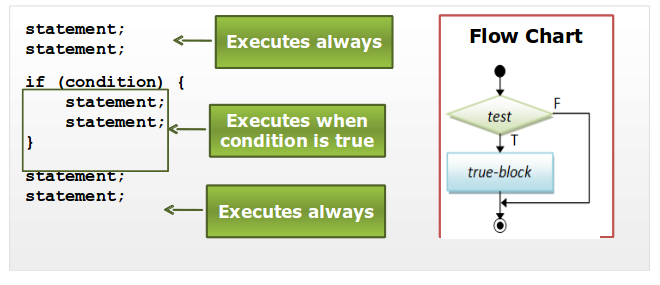
\includegraphics[scale=.45]{branching-if-syntax.png}   
 \end{center}
  \end{figure}
\end{frame}

\begin{frame}{Branching}
 \hspace{4cm}{22323020}
 
 \vspace{2pc}
Read the given number and call it X.

Divide X by 2 and record the remainder.

If remainder is 0, print ``X is even''.

Otherwise, print ``X is odd''.
\end{frame}

\begin{frame}[fragile]{Branching}
 \begin{lstlisting}[numbers=none]
public class EvenOdd {
    public static void main(String[] args) {
        int givenNumber = Integer.parseInt(args[0]);
        if (givenNumber % 2 == 0) {
            System.out.println("Number is even.");
        } else {
            System.out.println("Number is odd.");
        }
    }
}
 \end{lstlisting}
\end{frame}

\begin{frame}{Branching}
 \textbf{if-else Statement}
 
  The \lstinline!if-else! statement is a control flow statement that tells the program to execute a certain section of code. It depends on condition. If condition evaluates to true \lstinline!if! block is executed otherwise \lstinline!else! block.
  \begin{figure}[H]
   \begin{center}
    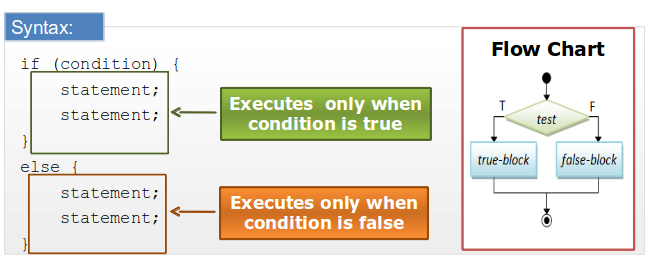
\includegraphics[scale=.45]{branching-if-else-syntax.png}
   \end{center}
  \end{figure}
\end{frame}

\begin{frame}{Branching}
 A Few More Operators
 
 \begin{description}
  \item [Arithmetic Operators] \%
  \item [Relational Operators] $<$ \hspace{.6cm}$>$ \hspace{.6cm}$<$= \hspace{.6cm}$>$= \hspace{.6cm}== \hspace{.6cm}!=
 \end{description}

 Can you name these operators and operations they perform on operands?
\end{frame}

\begin{frame}{Branching}
 \hspace{3cm}\textbf{Operator Description}
 \begin{tabular}{| p{1.8cm} | p{8.2cm} |}
  \hline
  operator & description \\ \hline
  == & Tests whether the expressions on the left and right are equivalent \\ \hline
  <= & Tests whether the expression on left less than or equal to the expression on right \\ \hline
  < & Tests whether the  expression on left less than the expression on right \\ \hline
  > & Tests whether the  expression on left greater than the expression on right \\ \hline
  >= & Tests whether the  expression on left greater than or equal to the expression on right \\ \hline
  != & Tests whether the expressions on the left and right are not equal \\ \hline
 \end{tabular}
\end{frame}

\begin{frame}{Branching}
 Be sure to distinguish between the relational operator == and the assignment operator =
 
 \vspace{1pc}
 \begin{description}
  \item [X == Y] Tests, if the contents of variable x are the same as the contents of variable y.
  \item [X = Y] Assigns the value stored in variable y to variable x (overwriting what is in x and leaving y unchanged)
 \end{description}

\end{frame}

\begin{frame}{Branching}
\begin{tabular}{l l}
\begin{minipage}{4cm}
\begin{block}{X == Y}
 9   ==  8
 
 a   ==  b
 
 a   ==  6
 
 5+6 ==  3+2
 
 5   ==  a
\end{block}
\end{minipage}
&
\begin{minipage}{4cm}
\begin{block}{X = Y}
 a = 8
 
 a = b
 
 a = 3+2
 
 \fbox{5  =  4 // Invalid}
\end{block}
\end{minipage}
\end{tabular}
\begin{block}{Note}
 When an operator has two characters (e.g. ==, <=, >= ), then there should be no space between them.
\end{block}
\end{frame}

\begin{frame}{Branching}
 Sequential and Branching statements
 
 \vspace{1pc}
 \textbf{Sequential Execution \hspace{1cm} Branching Execution}
 \begin{tabular}{l l}
\begin{minipage}{5cm}
\begin{figure}[H]
 \begin{center}
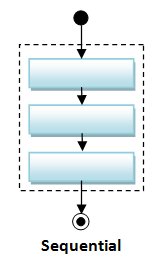
\includegraphics[scale=.5]{Branching-sequential-execution.png}  
 \end{center}

\end{figure}


\end{minipage}
&
\begin{minipage}{6cm}
\begin{figure}[H]
\centering
\begin{minipage}{2cm}
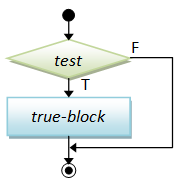
\includegraphics[scale=0.5]{branching-if-statement.png}
\caption*{If Statement}
\end{minipage}
\quad
\begin{minipage}{3cm}
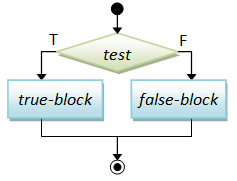
\includegraphics[scale=.6]{branching-ifelse-statement.png}
\caption*{If-else Statement}
\end{minipage}
\end{figure}
\end{minipage}
\end{tabular}
\end{frame}

\begin{frame}{Branching}
 Another problem involving Conditional Processing
 
 \begin{center}
 
\colorbox{gray}{\hspace{2.6cm} 4, 9\hspace{2.6cm}}

$\uparrow$
 
\colorbox{cyan}{Which is the largest number?}
  \end{center} 
\begin{block}{Solution}
\begin{itemize}
 \item Take the two numbers (n1, n2)
 \item If n1 is greater than n2, then n1 is largest.
 \item Otherwise, n2 is largest.
 \end{itemize}
\end{block}
 \end{frame}
 
 \begin{frame}{Branching}
  Let's Structure the Solution
  
  \vspace{1pc}
  
  n1 = First Number
  
  n2 = Second Number
  
  \lstinline!if (n1 > n2) print(``First number is larger'')!
  
  Otherwise, \emph{print(``Second number is larger'')}
  
 \end{frame}

\begin{frame}[fragile]{Branching}
 \begin{block}{Program to find largest among two numbers}
  \begin{lstlisting}[numbers=none]
public class LargerNumber {
    public static void main(String[] args) {
        int fNumber, sNumber;
        .........
        .........
        .........
    }
}
  \end{lstlisting}
 \end{block}
\end{frame}

\begin{frame}[fragile]{Branching}
 \begin{block}{Program to find largest among two numbers}
  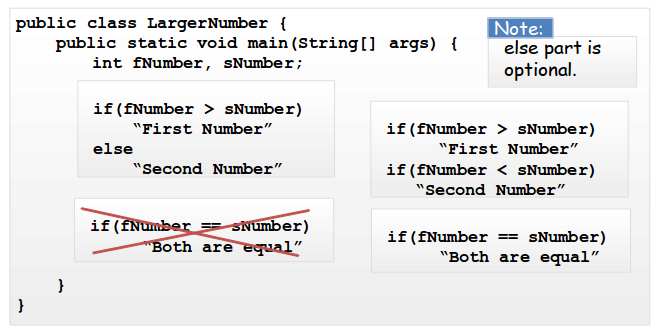
\includegraphics[scale=.45]{program-largest.png}
 \end{block}
What if \emph{fNumber} is equal to \emph{sNumber}? 
\end{frame}

\begin{frame}[fragile]{Branching}
 What are the problems with this code?
 
  \begin{lstlisting}[numbers=none]
public class LargerNumber {
    public static void main(String[] args) {
        int fNumber, sNumber;
        if (fNumber > sNumber) {
            "First Number"   
        } 
        else if(fNumber < sNumber) {
            "Second Number"
        } else {
            "Both are equal"
        }
    }
}
  \end{lstlisting}

\end{frame}

\begin{frame}{Branching}
 \begin{block}{First Problem}
  Second and third conditions are evaluated even if first condition is true
 \end{block}
 \begin{block}{Second Problem}
  If the first two conditions fail then no need test the third condition at all.
 \end{block}
 Is there any better way?
 \begin{center}
  
 \lstinline!if!...
 
 \lstinline!else if!...
 
 \lstinline!else!...
 \end{center}
\end{frame}

\begin{frame}{Branching}
 Syntax of \lstinline!if - else - if!
  \begin{figure}[H]
   \begin{center}
    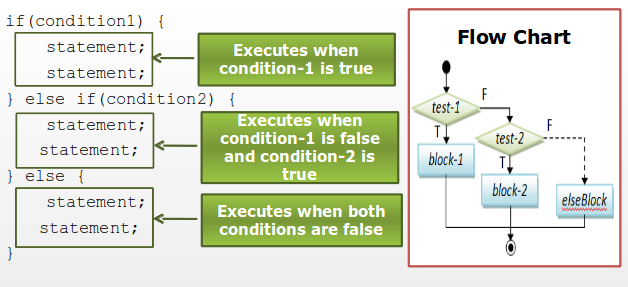
\includegraphics[scale=.5]{syntax-if-else-if.png}
   \end{center}

  \end{figure}

\end{frame}

\begin{frame}[fragile]{Branching}
 Write Java code to find largest among four numbers. The class name and basic structure  is given below:
 \begin{lstlisting}[numbers=none]
public class LargestNumber {
    public static void main(String[] args) {
        int next, largestSoFar;
        .........
        .........
        .........
    }
}  
 \end{lstlisting}

\end{frame}

\begin{frame}[fragile]{Branching}
Write a Java program to find the grade of a student (given the marks) using the following rules. Print ``Marks: Grade''
91-100: A grade; 81-90: B grade; 71-80: C grade; 
61-70: D grade; 51-60: E grade;  < 51: Fail

\begin{lstlisting}[numbers=none]
public class StudentGrade {
    public static void main(String[] args) {
        int marks = Integer.parseInt(args[0]);
        .........
        .........
        .........
    }
}
\end{lstlisting}
\end{frame}

\begin{frame}[fragile]{Branching}
 Given two numbers, print `true' if they are equal; `false' otherwise.
 \begin{lstlisting}[numbers=none]
public class TwoNumsEqual {
    public static void main(String[] args) {
        ....
        ....
        if (num1 == num2)
            System.out.print ("true");
        else
            System.out.print ("false");
    }
}
 \end{lstlisting}
\end{frame}

\begin{frame}[fragile]{Branching}
\textbf{Add Elegance to the Code}

Can we write the code more elegantly?

\begin{block}{Try this}
 \begin{lstlisting}[numbers=none]
public class TwoNumsEqual {
    public static void main(String[] args) {
        ....
        System.out.print(num1 == num2);
    }
}
 \end{lstlisting}
\end{block}
\end{frame}

\begin{frame}[fragile]{Branching}
 \begin{block}{Nested If}
  Let's see how we can write a solution to find the smallest number among three numbers:
 \end{block}
\begin{minipage}{5.3cm}
 \begin{lstlisting}[numbers=none, frame=single]
if (n1 < n2)  
    if (n1 < n3)  
        n1 is smallest
    else  			
        n3 is smallest
else  // n2 is smaller than n1
    if (n2 < n3)  
        n2 is smallest
    else 
        n3 smallest   	
 \end{lstlisting}
\end{minipage}
\quad
\begin{minipage}{4.7cm}
 \begin{lstlisting}[numbers=none,frame=single]
if ((n1 < n2) && (n1 < n3))
    n1 is smallest
else if (n2 < n3)
    n2 is smallest
else
    n3 is smallest
 \end{lstlisting}

\end{minipage}
\end{frame}

\begin{frame}[fragile]{Branching}
 Now, if we want to find largest among four numbers:
 
 \begin{center}
 
\colorbox{gray}{\hspace{2.3cm}4, 9, 2, -27\hspace{2.3cm}}

$\uparrow$
 
\colorbox{cyan}{Which is the largest number?}
  \end{center} 
 So, how many levels of nested condition do we have to write?
 
Or, how many conditions do we have to logically combine? 
\end{frame}

\begin{frame}[fragile]{Branching}
 \begin{lstlisting}[numbers=none]
n1 = Integer.parseInt(args[0]);
n2 = Integer.parseInt(args[1]);
n3 = Integer.parseInt(args[2]);
n4 = Integer.parseInt(args[3]);
if ((n1 > n2) && (n1 > n3) && (n1 > n4))
    n1 is largest
else if ((n2 > n3) && (n2 > n4))
    n2 is largest
else if ((n3 > n4))
    n3 is largest
else
    n4 is largest
 \end{lstlisting}

\end{frame}

\begin{frame}[fragile]{Branching}
 Solution ? Use an intermediate variable.
 
 \vspace{1pc}
 n1 = First Number
 
 n2 = Second Number
 
 \lstinline!if (n1 > n2) largestSoFar = n1;  otherwise, largestSoFar = n2;!
 
 n3 = Third Number
 
 \lstinline!if (n3 > largestSoFar) largestSoFar = n3!
 
 n4 = Fourth Number
 
 \lstinline!if (n4 > largestSoFar) largestSoFar = n4!
 
 Print \textbf{largestSoFar}
  
\end{frame}

\begin{frame}[fragile]{Branching}
  We can do even better. Because we need only one of \texttt{n1, n2, n3} and \texttt{n4} at anytime, we can use only one variable for all the four numbers, holding them one at a time. 
  
  \vspace{1cm}
  largestSoFar = First Number
  
  next = Second Number
  
  \lstinline!if (next > largestSoFar) largestSoFar = next!
\end{frame}

\begin{frame}[fragile]{Branching}
 next = Third Number
 
 \lstinline!if (next > largestSoFar) largestSoFar = next!
 
 next = Fourth Number
 
 \lstinline!if (next > largestSoFar) largestSoFar = next!
 
 Print \textbf{largestSoFar}
\end{frame}

\begin{frame}[fragile]{Branching}
 Use an intermediate variable called grade and see how it helps.
 \begin{lstlisting}[numbers=none]
public class StudentGrade {
    public static void main(String[] args) {
        char grade;
        .........
        .........
        .........
    }
}
 \end{lstlisting}

\end{frame}


\begin{frame}{Branching}
 \begin{figure}[H]
 \begin{center}
   
\includegraphics[scale=.3]{qa.png}   
 \end{center}
  \end{figure}
\end{frame}



\end{document}

